\section{Dust Empirical Modeling} \label{sec:methods}
\subsection{Fiducial DEM} 
\todo{motivation for the DEM model} 

We begin by defining the dust attenuation curve $A(\lambda)$ as 
\begin{equation} 
    F_o (\lambda) = F_i (\lambda) 10^{-0.4 A(\lambda)}
\end{equation}
where $F_o$ is the observed flux and $F_i$ is the intrinsic flux. We normalize the attenuation at the $V$ band, 
\begin{equation} 
    A(\lambda) = A_V \frac{k(\lambda)}{k_V}. 
\end{equation}


For the normalization of the attenuation curve, $A_V$, we use the slab model
from~\cite{somerville1999, somerville2012}. In the slab model the amplitude of
attuenuation depends on the inclination angle, $i$, and the optical depth,
$\tau_V$: 
\begin{equation} 
    A_V = -2.5 \log \left[ \frac{1 - e^{-\tau_V\,\sec i}}{\tau_V\,\sec i} \right]
\end{equation}
\todo{justification of why this is enough}. We sample $i$ uniformly.

Recently, \cite{salim2020} find significant dependence in $A_V$ on both $M_*$
and SFR. We include this dependence through $\tau_V$, which we flexibly
parameterize as 
\begin{equation}
    \tau_V(M_*, {\rm SFR}) = m_{\tau,1} \log \left(\frac{M_*}{10^{10} M_\odot}\right) +
    m_{\tau,2} \log\,{\rm SFR} + c_\tau.
\end{equation}

Next, for the wavelength dependence of the attenuation curve, we use $k(\lambda)$ from 
\cite{noll2009}: 
\begin{equation}
    k(\lambda) = \left(k_{\rm Cal}(\lambda) + D(\lambda)\right) \left(
    \frac{\lambda}{\lambda_V} \right)^\delta.
\end{equation}
Here $k_{\rm Cal}(\lambda)$ is the \cite{calzetti2001} curve: 
\[
    k_{\rm Cal}(\lambda) = 
    \begin{cases} 
        2.659 (-1.857 + 1.040/\lambda) + R_V, & 6300 \AA \le \lambda \le
        22000 \AA \\ 
        2.659 (-2.156 + 1.509/\lambda - 0.198/\lambda^2 + 0.011/\lambda^3) +
        R_V & 1200 \AA \le \lambda \le 6300 \AA
    \end{cases}
\]
where $\lambda_V$ is the $V$ band wavelength. $\delta$, the slope of the attenuation curve.
also correlates with galaxy
properties.
So we parameterize $\delta$ and 
\begin{align}
    \delta(M_*, {\rm SFR}) &= m_{\delta,2} \log \left(\frac{M_*}{10^{10}
    M_\odot}\right) + m_{\delta,2} \log\,{\rm SFR} + c_\delta 
\end{align}

$D(\lambda)$ is the UV dust bump, which we
parameter using the standard Lorentzian-like Drude profile:
\begin{equation}
    D(\lambda) = \frac{E_b(\lambda \Delta \lambda)^2}{(\lambda^2 -
    \lambda_0^2)^2 + (\lambda \Delta \lambda)^2}
\end{equation}
where $\lambda_0$, $\Delta \lambda$, and $E_b$ are the central wavelength,
FWHM, and strength of the bump, respecitvely. In our DEM, we assume fixed 
$\lambda_0 = 2175 \AA$ and $\Delta \lambda = 350\AA$. 

\cite{kriek2013} and \cite{tress2018} found evidence that $E_b$ correlates with
the slope of the attenuation curve for star-forming galaxies $z\sim2$. This was
dependence was confirmed with simulations in \cite{naranyanan2018}. $E_b$: 
\begin{align}
    E_b &= m_E~\delta + c_E
\end{align}

We also split the attenuation on the star light and nebular emission 
\begin{equation} 
    F_o (\lambda) = F^{\rm star}_i (\lambda) 10^{-0.4 A(\lambda)} + F^{\rm
    neb}_i (\lambda) 10^{-0.4 A_{\rm neb}(\lambda)}
\end{equation}
where we parameterize
\begin{equation}
    A_{\rm neb}(\lambda) = f_{\rm neb}  A(\lambda) 
\end{equation} 

\todo{mention of how we treat SFR = 0 galaxies} 

\begin{figure}
\begin{center}
    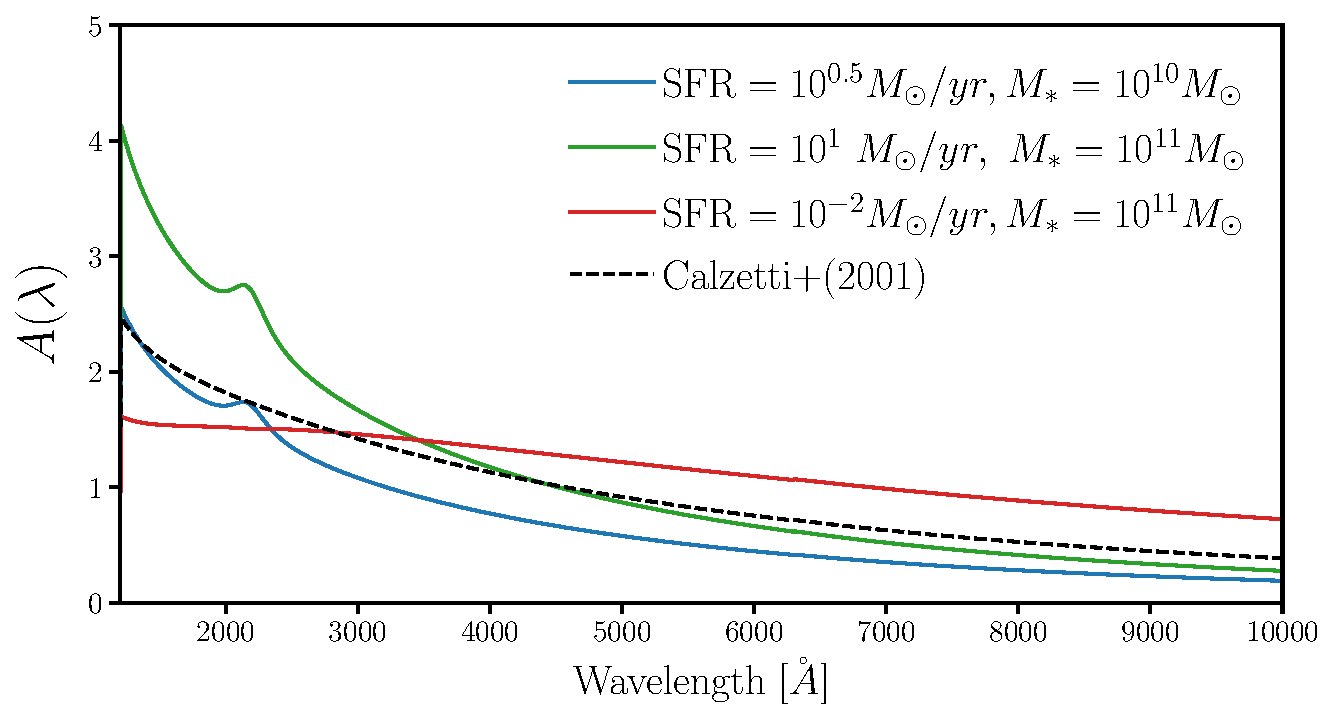
\includegraphics[width=0.9\textwidth]{figs/dems.pdf}
    \caption{comparison of fiducial DEM to attenuation curve in the literature.}
\label{fig:dem}
\end{center}
\end{figure}


\subsection{Beyond the Slab DEM}  \label{sec:nonslab} 
A major assumption of our fiducial DEM is that we sample the amplitude of
attenuation from the slab model. The slab model makes a strong simplifying 
assumption that the dust in galaxies \todo{details}. \todo{sentence or two
about how we know the slab model doesn't work}. 

Furthermore, the slab model predicts $A_V$ distribution significantly different
than $A_V$ distributions measured from observations. In Figure~\ref{fig:av_dist}, we compare the $A_V$
distribution predicted by the slab model for $\tau_V = $ to the $A_V$ 
distribution of SDSS galaxies from \cite{brinchmann2004}. The comparison clearly reveals the
discrepancy between the SDSS $A_V$ distribution and the slab model prediction.
The slab model predicts a sharp cutoff at lower $A_V$ end of the distribution,
which is not found in observables. 
The SDSS $A_V$ measurements can be negative in \cite{brinchmann2004} because 
\todo{...}. 


To ensure that our results do not depend significantly on the slab
model, we implement a more flexible alternative model for sampling $A_V$ based on a
truncated normal distribution: 
\begin{equation}
    A_V \sim \mathcal{N}_T(\mu_{A_V}, \sigma_{A_V}) =
    \frac{\mathcal{N}(\mu_{A_V}, \sigma_{A_V})}{1 -
    \Phi\left(-\frac{\mu_{A_V}}{\sigma_{A_V}}\right)}.
\end{equation}
$\mathcal{N}$ is the standard normal distribution and $\Phi$ is the cumulative
distribution function of the standard normal distribution function.
$\Phi(x) = \frac{1}{2}(1+{\rm erf}(x/\sqrt{2})$. $\mu_{A_V}$ and $\sigma_{A_V}$
are the mean and variance of the truncated normal distribution. 
\todo{There}




%%%%%%%%%%%%%%%%%%%%%%%%%%%%%%%%%%%%%%%%%%
% table of free parameters
%%%%%%%%%%%%%%%%%%%%%%%%%%%%%%%%%%%%%%%%%%
\begin{table}
    \caption{Free Parameters of the Dust Empirical Model} 
    \begin{center}
        \begin{tabular}{cc} \toprule
            Parameter & Definition \\[3pt] \hline\hline
            $m_{\tau,1}$ & Slope of the $\log M_*$ dependence of optical depth, $\tau_V$\\
            $m_{\tau,2}$ & Slope of the $\log {\rm SFR}$ dependence of optical depth, $\tau_V$\\
            $c_{\tau}$ & amplitude of the optical depth, $\tau_V$\\
            $m_{\delta,1}$ & Slope of the $\log M_*$ dependence of the attenuation curve slope, $\delta$\\
            $m_{\delta,2}$ & Slope of the $\log {\rm SFR}$ dependence of the attenuation curve slope, $\delta$\\
            $c_{\delta}$ & amplitude of the attenuation curve slope, $\delta$\\
            $m_{E}$ & slope of the $\delta$ dependence of UV dust bump strength, $E_b$\\
            $c_{E}$ & amplitude of UV dust bump strength, $\delta$\\
            $f_{\rm neb}$ & fraction of nebular attenuation curve\\
            \hline
        \end{tabular} \label{tab:free_param}
    \end{center}
\end{table}
%%%%%%%%%%%%%%%%%%%%%%%%%%%%%%%%%%%%%%%%%%

\subsection{Likelihood-Free Inference} 
Approximate Bayesian Computation with Population Monte Carlo \cite{hahn2017a},

discussion of observables and distance metric 
\cite{ishida2015} 

Paragraph on the priors we choose. 

\begin{figure}
\begin{center}
    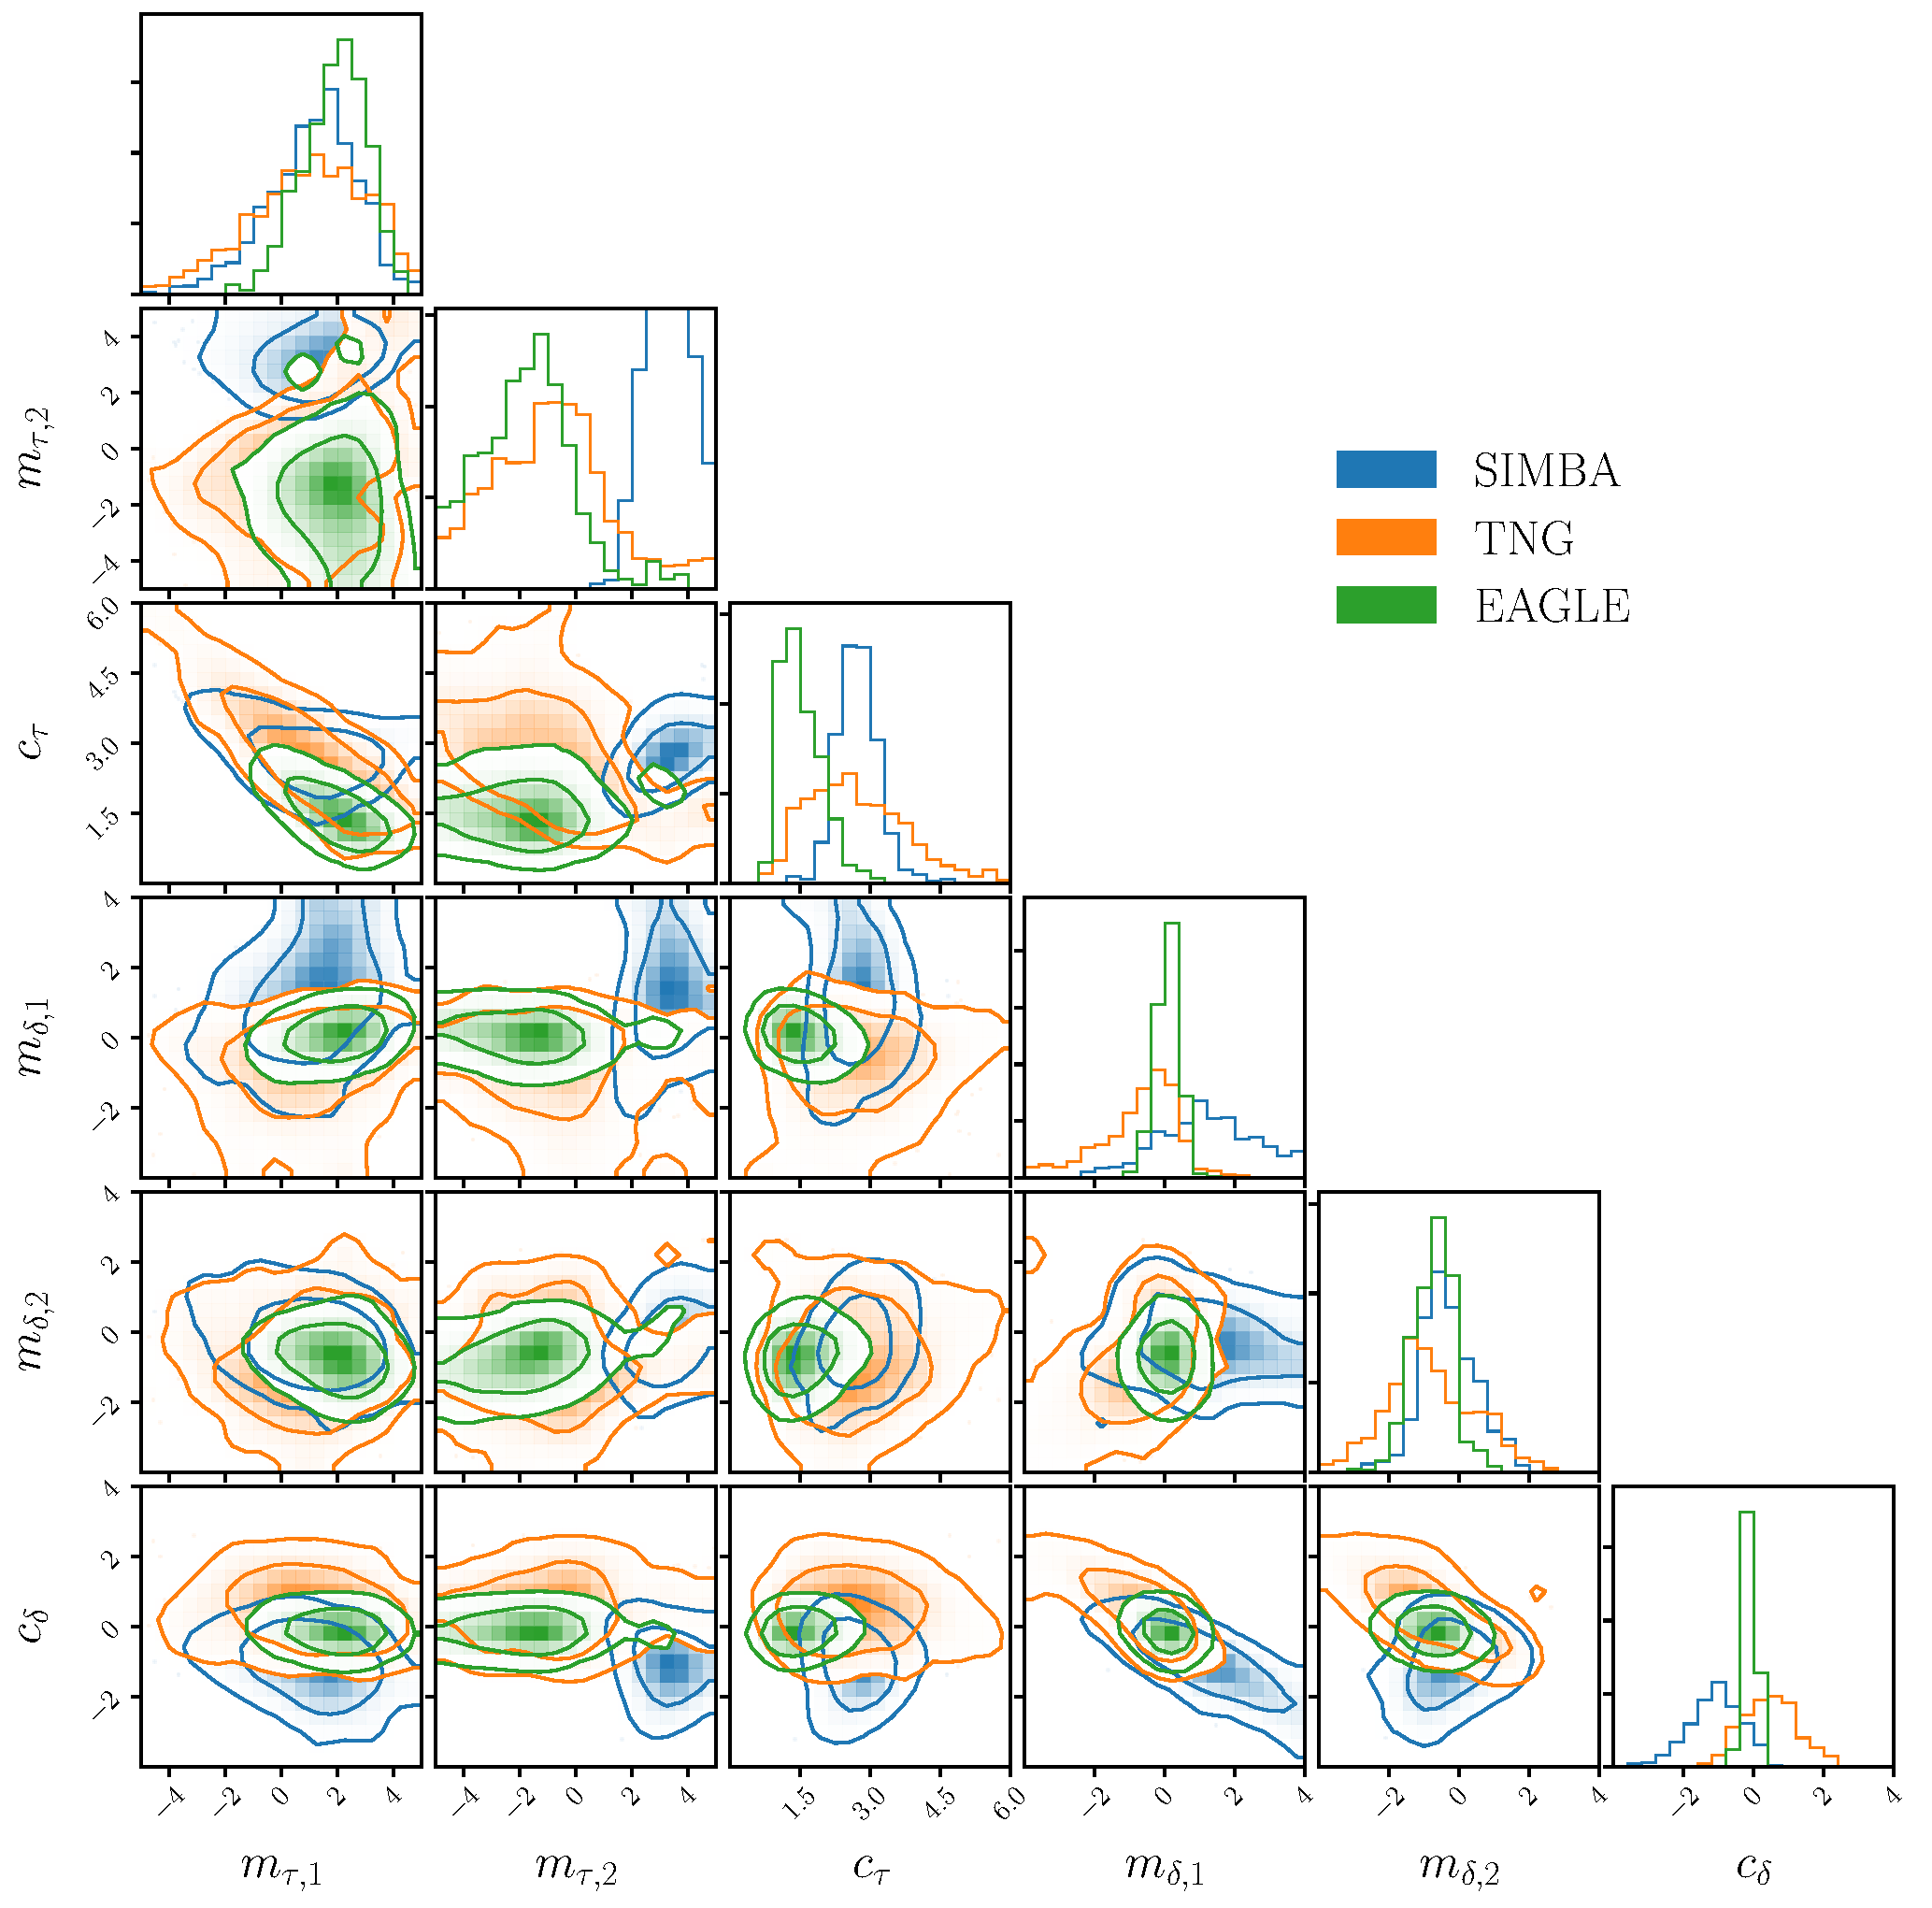
\includegraphics[width=\textwidth]{figs/abc.pdf}
    \caption{Posterior of the DEM parameters.}
\label{fig:dem}
\end{center}
\end{figure}

\begin{figure}
\begin{center}
    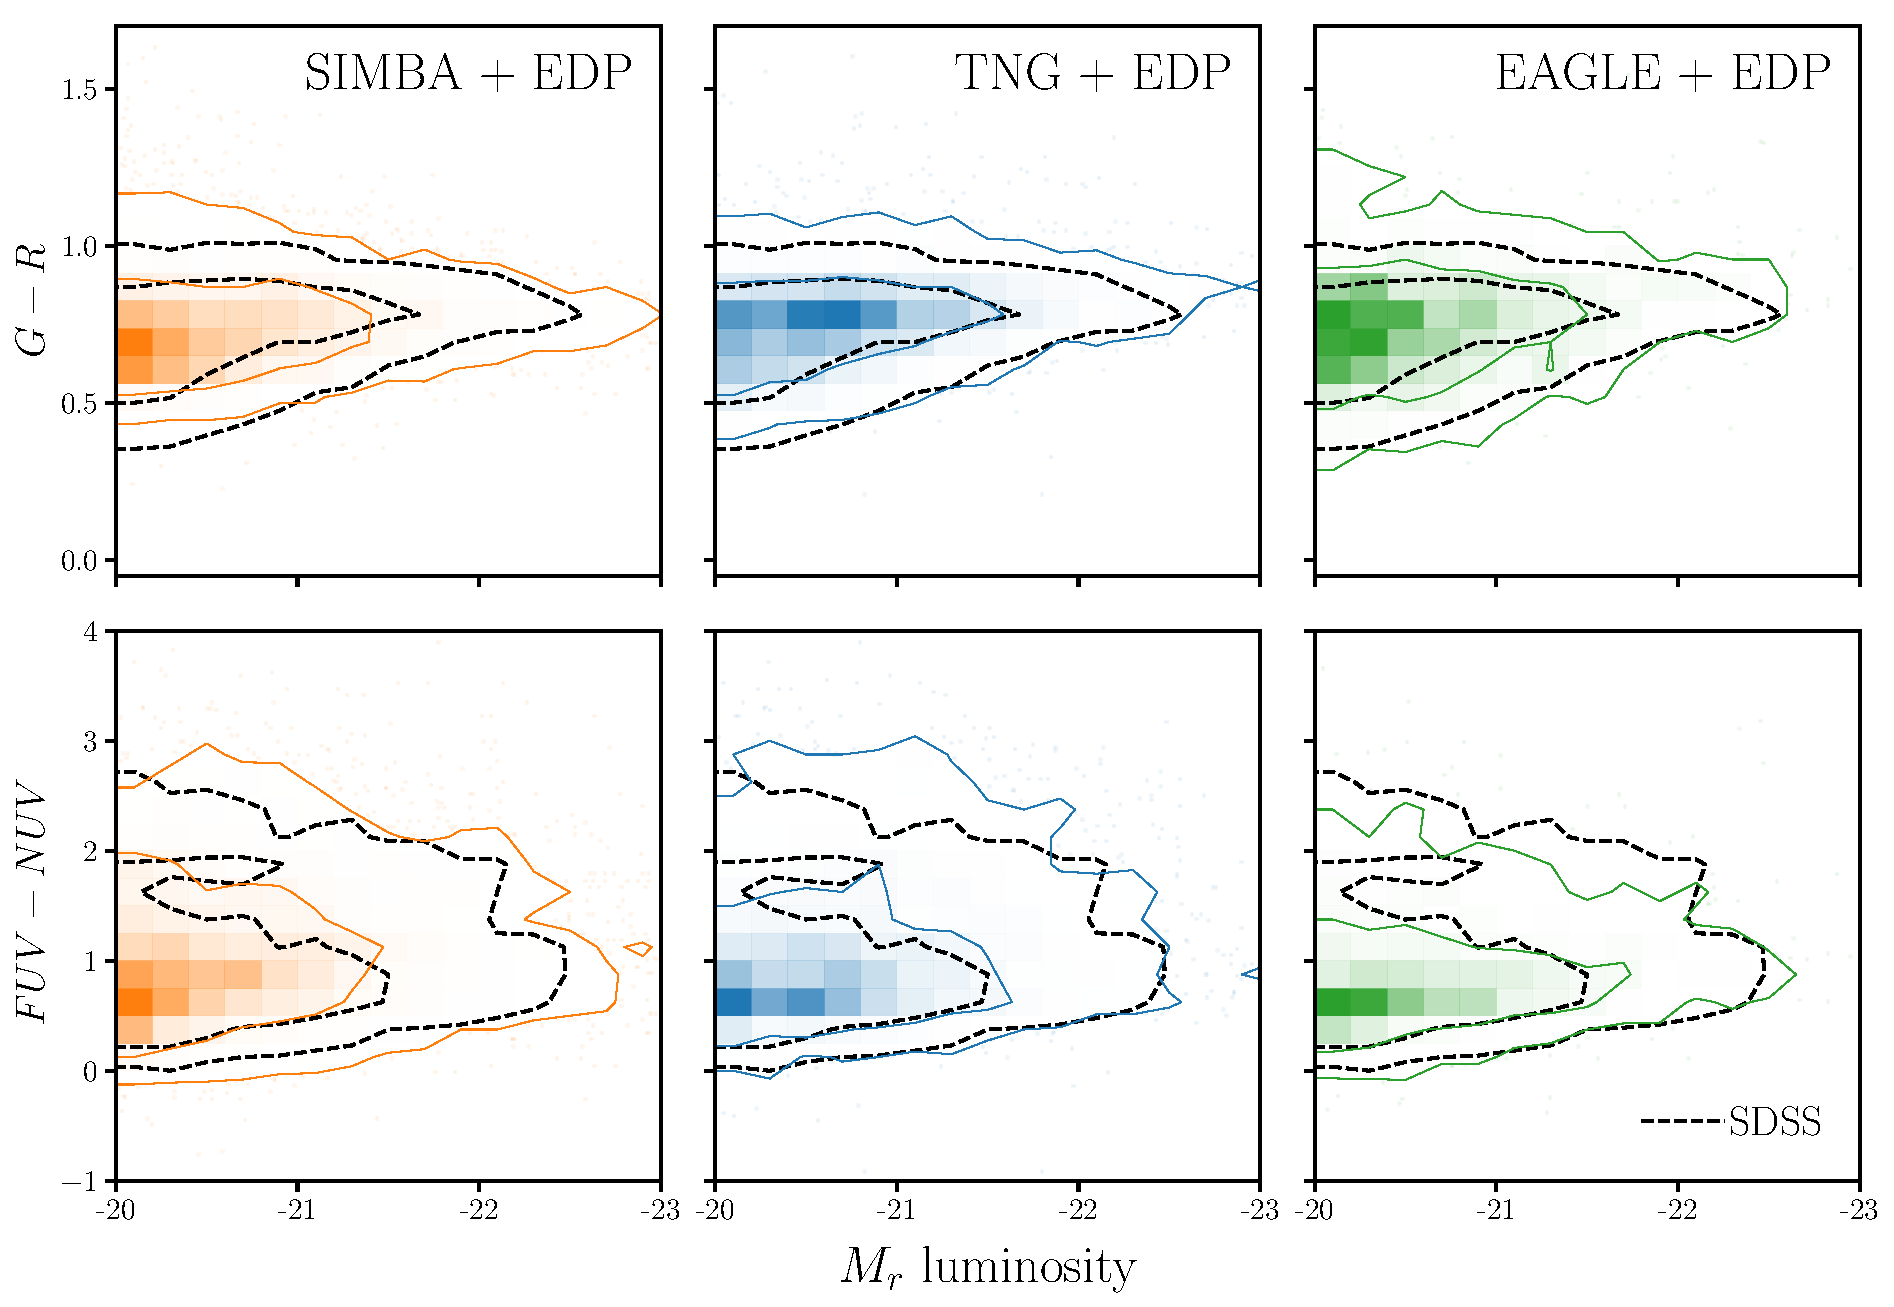
\includegraphics[width=\textwidth]{figs/abc_observables.pdf}
    \caption{Comparison of the observables predicted by the simulations with
    the posterior DEM.}
\label{fig:dem}
\end{center}
\end{figure}
